\documentclass{article}

%-------------------------------------------------

\usepackage{fullpage}

\usepackage{graphicx}

\usepackage{amsmath}
\usepackage{amssymb}
\usepackage{amsfonts}

\usepackage{color}

\usepackage{verbatim}

\usepackage{tikz}
\usetikzlibrary{arrows,automata}

%-------------------------------------------------

\newcommand{\FIXME}[1]{\textcolor{red}{\textbf{#1}}}

%-------------------------------------------------

\newcommand{\stdin}{\texttt{stdin}~}
\newcommand{\stdout}{\texttt{stdout}~}
\newcommand{\stderr}{\texttt{stderr}~}

\newcommand{\PID}{\texttt{PID}~}

\newcommand{\multiprocessing}{\texttt{multiprocessing}~}
\newcommand{\multiprocessingConnection}{\texttt{multiprocessing.Connection}~}

\newcommand{\GraceDB}{\texttt{GraceDB}~}
\newcommand{\alert}{\texttt{lvalert}~}

\newcommand{\lvalertListen}{\texttt{lvalert\_listen}~}
\newcommand{\lvalertSend}{\texttt{lvalert\_send}~}

\newcommand{\lvalertMP}{\texttt{lvalertMP}~}
\newcommand{\lvalertListenMP}{\texttt{lvalert\_listenMP}~}
\newcommand{\lvalertCommandMP}{\texttt{lvalert\_commandMP}~}

\newcommand{\interactiveQueue}{\texttt{interactiveQueue}~}
\newcommand{\parseAlert}{\texttt{parseAlert}~}

\newcommand{\SortedQueue}{\texttt{SortedQueue}~}
\newcommand{\QueueItem}{\texttt{QueueItem}~}
\newcommand{\Task}{\texttt{Task}~}

\newcommand{\lvalertMPini}{\texttt{lvalert\_listenMP.ini}~}
\newcommand{\childConfigini}{\texttt{childConfig.ini}~}

\newcommand{\approvalProcessor}{\texttt{approval\_processor}~}
\newcommand{\eventSupervisor}{\texttt{event\_supervisor}~}

%-------------------------------------------------
\begin{document}
%-------------------------------------------------

\title{
\lvalertMP User's Guide
}

\author{
Reed Essick \\
reed.essick@ligo.org
}

\maketitle

\newpage

%------------------------

\tableofcontents
\listoffigures

\newpage

%------------------------

\section{introduction}

\lvalertListen provides an extremely flexible infrastructure from which processes can listen and respond to events within \GraceDB. 
However, it currently only communicates with the forked process once (via \stdin) and therefore cannot send multiple \alert messages to any procesess.
For most follow-up, this is not an issue.
Many processes simply respond to any new event which passes a basic FAR threshold. 
However, a few key processes will benefit from receiving all alerts about a set of events.
Indeed, passing all \alert messages to a single process obviates the inter-process communication and associated race conditions that would be required of multiple independent processes, each forked with a separate, single \alert message.

This guide describes how \lvalertListenMP addresses and resolves this problem. 
In particular, we focus on a pedagogical description of the classes and methods used within the executables.
We also focus on the user's interface with the tools from the command line.

Briefly, \lvalertListenMP uses the same interface with the \alert servers as \lvalertListen but forks child processes via Pythons multiprocessing module.
In this way, \lvalertListenMP can communciate with the child processes repeatedly (through a shared \multiprocessingConnection object).
The module provides a standardized way to schedule and execute follow-up activities.
While the actual follow-up implemented here is basic, it is easily extended to achieve more complicated goals.
An example is the \eventSupervisor library.

This guide is organized as follows. In \S\ref{sec: classes, methods, configs and executables}, we enumerate and describe the basic objects, methods, configuration files, and executables defined within this module. 
This includes examples for how these might be used.
In \S\ref{sec: workflow}, we demonstrate the workflow within \lvalertListenMP and describe how the various parts work together to manage follow-up tasks.
Finally, we discuss existing and suggested extensions in \S\ref{sec: suggested extensions}.

%------------------------

\section{classes, methods, configs and executables}
\label{sec: classes, methods, configs and executables}

This section defines the classes (\S\ref{sec: classes}), methods (\S\ref{sec: methods}), configuration files (\S\ref{sec: configs}), and executables (\S\ref{sec: executables}) that are necessary for \lvalertListenMP to function. 
Their interactions are described in \S\ref{sec: workflow}, so we focus on the particular responsibilities associated with each element here.

%-----------

\subsection{classes}
\label{sec: classes}

There are three (3) main classes defined within \lvalertMP:
\begin{itemize}
    \item{\SortedQueue (\S\ref{sec: SortedQueue})}
    \item{\QueueItem (\S\ref{sec: QueueItem})}
    \item{\Task (\S\ref{sec: Task})}
\end{itemize}
These objects are what allow \lvalertListenMP to define and schedule multiple follow-up activities based on \alert messages about multiple events within a single process.
In particular, individual activities are encapsulated as \Task objects.
Each \QueueItem is associated with one or more \Task objects.
\SortedQueue contains an ordered list of \QueueItem instances, and when each \QueueItem \textit{expires} the activities associated therewith are accomplished through a call to \QueueItem.execute(), which in turn delegates to \Task.execute() for each associated \Task instance as needed.
Futhermore, \QueueItem instances posses the concept of ``completion'' and will label themselves as ``completed'' when all their \Task instances have been run or are otherwise satisfied.

%---

\subsubsection{\SortedQueue}
\label{sec: SortedQueue}

The \SortedQueue class is a simple wrapper around a Python \texttt{list} that manages the order of the elements within the \texttt{list}.
We require all elements to be a subclass of \QueueItem and so ensure that each element has a notion of \textit{expiration} and \textit{completion}.
Furthermore, \SortedQueue supports a few basic \texttt{list} manipulations and queries.

\vspace{0.5cm}
\noindent
\textit{attributes}

\begin{itemize}
    \item{queue [\texttt{list}]
        \begin{itemize}
            \item{a Python \texttt{list} which stores the \QueueItem instances. \SortedQueue orders the elements of this \texttt{list} and provides some high level interface functionality to manipulate them.}
        \end{itemize}
         }
\end{itemize}

\noindent
\textit{methods}

\begin{itemize}
    \item{\_\_init\_\_()
        \begin{itemize}
            \item{basic instantiation. Sets the \textit{queue} attribute to an empty list.}
        \end{itemize}
         }
    \item{\_\_len\_\_()
        \begin{itemize}
            \item{returns the length of the \texttt{list} stored as the \textit{queue} attribute.}
        \end{itemize}
         }
    \item{\_\_getitem\_\_(ind [\texttt{int}])
        \begin{itemize}
            \item{returns the element of \textit{queue} corresponding to a specified index.}
        \end{itemize}
         }
    \item{insert(newItem [\QueueItem])
        \begin{itemize}
            \item{inserts the new \QueueItem into \textit{queue} in the correct order. This is done through a direct iteration over \textit{queue} and could be sped up by representing \textit{queue} with a better data structure. Also checks that newItem is a sublcass of \QueueItem.}
        \end{itemize}
         }
    \item{pop(ind=0 [\texttt{int}])
        \begin{itemize}
            \item{removes and returns the \QueueItem corresponding the the specified index. The default is to return the first item in \textit{queue}.}
        \end{itemize}
         }
    \item{clean()
        \begin{itemize}
            \item{removes all \QueueItem instances marked as \textit{complete} from \textit{queue}. This allows us to simply modify an attribute of a \QueueItem upon execution or during \parseAlert (\S\ref{sec: parseAlert}) and let the \SortedQueue clean up all completed items periodically.}
        \end{itemize}
         }
\end{itemize}


%---

\subsubsection{\QueueItem}
\label{sec: QueueItem}

The \QueueItem class encapsulates the idea of a single follow-up process.
Each processes may be required to do several things and must order or schedule those things internally.
\QueueItem instances accomplish this by storing two \texttt{list}s of \Task objects, with each \Task respresenting a single activity.
As the \Task instances are completed (via delegation through \Task.execute), they are shuffled from the \textit{tasks} list to the \textit{completedTasks} list.
\QueueItem's also contain the concepts of \textit{expiration} (when the next \Task should be executed) as well as \textit{completion} (whether there are more tasks to be completed).
We note that the internal storage of ordered \Task instances within the \QueueItem is similar to the ordered storage within \SortedQueue instances.
If desired, multiple \Task instances can be scheuduled and managed with \SortedQueue alone by assigning a single \Task to each \QueueItem and filling the \SortedQueue with multiple \QueueItem instances.
However, we allow \QueueItem instances to manage multiple tasks because this can sometimes simplify the representation of single follow-up processes.

\vspace{0.5cm}
\noindent
\textit{attributes}

\begin{itemize}
    \item{name [\texttt{str}]
        \begin{itemize}
            \item{usef for look-up because it can be more vonvenient than type-checking. \eventSupervisor uses the \textit{name} attribute to extract sections from it's config file. This should be overwritten by any extension.}
        \end{itemize}
         }
    \item{description [\texttt{str}]
        \begin{itemize}
            \item{a simple string describint what the \QueueItem is meant to do. Should be overwritten by any extension.}
        \end{itemize}
         }
    \item{t0 [\texttt{float}]
        \begin{itemize}
            \item{the reference time from which expiration will be set in \Task instances.}
        \end{itemize}
         }
    \item{tasks [\texttt{list}]
        \begin{itemize}
            \item{a list of \Task instances, not necessarily ordered (ordering is managed internally), which will be manaaged within the \QueueItem.}
        \end{itemize}
         }
    \item{completedTasks [\texttt{list}]
        \begin{itemize}
            \item{a list of \Task instances that have already been run by \QueueItem.execute(). Instantiated as an empty list.}
        \end{itemize}
         }
    \item{expiration [\texttt{float}]
        \begin{itemize}
            \item{reflects the earlieste expiration of all uncomplted \Task instances associated with this \QueueItem. Used to determin \QueueItem's placement within \SortedQueue.}
        \end{itemize}
         }
\end{itemize}

\noindent
\textit{methods}

\begin{itemize}
    \item{\_\_init\_\_(t0 [\texttt{float}], tasks [\texttt{list}])
        \begin{itemize}
            \item{basic instantiation. Set's \Task's expiration by referencing \textit{t0}.}
        \end{itemize}
         }
    \item{sortTasks()
        \begin{itemize}
            \item{ensure \textit{tasks} is ordered by expiration. Also, updates \QueueItem.expiration}
        \end{itemize}
         }
    \item{hasExpired()
        \begin{itemize}
            \item{checks whether \QueueItem needs attention by comparing time.time() to \QueueItem.expiration.}
        \end{itemize}
         }
    \item{execute(verbose=False [\texttt{bool}])
        \begin{itemize}
            \item{iteratively executes all \Task instances in \textit{tasks} that have expired and updates internal storage accordingly.}
        \end{itemize}
         }
    \item{add(newTasks [\texttt{list}])
        \begin{itemize}
            \item{adds a new \Task to the \QueueItem and updates attributes accordingly.}
        \end{itemize}
         }
    \item{remove(taskName [\texttt{str}])
        \begin{itemize}
            \item{removes and returns the first \Task within \textit{tasks} with \Task.name == taskName. If no such \Task exists, raises a \texttt{KeyError}.}
        \end{itemize}
         }
\end{itemize}

%---

\subsubsection{\Task}
\label{sec: Task}

Each \Task represents one follow-up activity.
Each follow-up process may perform multiple activities and therefore correspond to multiple \Task objects.
These are grouped together under a single \QueueItem instance for each follow-up process.

\Task instances perform the actual follow-up activities through delegation to their \textit{functionHandle} attributes.
There is a standardized input argument format for \textit{functionHandle} calls which is followed by the \Task.execute call.
This can be changed and/or modified by creating an extension of the \Task and overwriting the execute method.

\Task objects also contain the concept of \textit{timing out} and \textit{expiration}.
When they are instantiated, they only know of their \textit{timeout}, or the number of seconds (after some reference time) which must ellapse before they should be executed.
When the \textit{setExpiration} method is called, the \textit{expiration} is computed using the supplied reference time to compute a time-stamp.
Note, if we can call \textit{setExpiration} repeatedly if needed.

\vspace{0.5cm}
\noindent
\textit{attributes}

\begin{itemize}
    \item{name [\texttt{str}]
        \begin{itemize}
            \item{used for look-up and can be simpler than type-checking. Should be overwritten by any extension.}
        \end{itemize}
         }
    \item{description [\texttt{str}]
        \begin{itemize}
            \item{a prose statement describing what the \Task is supposed to do. Should be overwritten by any extension.}
        \end{itemize}
         }
    \item{timeout [\texttt{float}]
        \begin{itemize}
            \item{the amount of time (relative to some reference) that must ellapse befor the \Task needs attention.}
        \end{itemize}
         }
    \item{expiration [\texttt{float}]
        \begin{itemize}
            \item{the time-stamp for when this \Task needs attention. Instantiated as \texttt{None} and set with \textit{setExpiration}.}
        \end{itemize}
         }
    \item{functionHandle [\texttt{method}]
        \begin{itemize}
            \item{a method which is called from within \Task.execute(). Must take a standardized input argument with signature: \textit{functionHandle(verbose=verbose, *args, **kwargs)}.}
        \end{itemize}
         }
    \item{args [\texttt{list}]
        \begin{itemize}
            \item{extra argments for \textit{functionHandle}}
        \end{itemize}
         }
    \item{kwargs [\texttt{dict}]
        \begin{itemize}
            \item{extra keyword arguments for \textit{functionHandle}}
        \end{itemize}
         }
\end{itemize}

\noindent
\textit{methods}

\begin{itemize}
    \item{\_\_init\_\_(timeout [\texttt{float}], functionHandle [\texttt{method}], *args, **kwargs)
        \begin{itemize}
            \item{sets \textit{expiration} to \texttt{None} and stores data.}
        \end{itemize}
         }
    \item{setExpiration(t0 [\texttt{float}])
        \begin{itemize}
            \item{computes \textit{expiration = t0+timeout}}
        \end{itemize}
         }
    \item{hasExpired()
        \begin{itemize}
            \item{compares time.time() to \textit{expiration} to determine whether \Task needs attention.}
        \end{itemize}
         }
    \item{execute( verbose=False [\texttt{bool}])
        \begin{itemize}
            \item{delegates to \textit{functionHandle} with signature: \texttt{return self.functionHandle( verbose=verbose, *args, **kwargs )}}
        \end{itemize}
         }
\end{itemize}

%-----------

\subsection{methods}
\label{sec: methods}

There are two (2) main methods defined within \lvalertMP. 
\begin{itemize}
    \item{\interactiveQueue (\S\ref{sec: interactiveQueue})}
    \item{\parseAlert (\S\ref{sec: parseAlert})}
\end{itemize}
\interactiveQueue is called form within \lvalertListenMP via \multiprocessing and assigned a separate \PID.
Therefore, \interactiveQueue handles most of the manipulations of \SortedQueue instances and execution.
\parseAlert is called from within \interactiveQueue whenever a new \alert message is detected in the \multiprocessingConnection.
These \alert messages are passed from \lvalertListenMP to \interactiveQueue through the \multiprocessingConnection (\S\ref{sec: workflow}), and then \parseAlert is called to manipulate the \SortedQueue's as needed.
Thus, \parseAlert contains the acutal logic for how the follow-up should behave.
For this reason, any extension will need to define it's own \parseAlert method to control how it behaves.

Note: if \interactiveQueue raises an exception or otherwise terminates, \lvalertListenMP will also terminate.
Event if it is managing multiple \interactiveQueue instances, all of them will be terminated as \lvalertListenMP exits.
Thus, if anything fails it all fails in an effort to avoid small problems from propagating or going undetected.

%---

\subsubsection{\interactiveQueue}
\label{sec: interactiveQueue}

A persistent loop that listens for new \alert messages and checks if \QueueItem instances stored in a \SortedQueue need attention. 
Manages \textit{queue} through delegation to \parseAlert and execution through \QueueItem.execute(). 
Loads libraries baes on the \texttt{process\_type} option in the \childConfigini, which is currently hard coded to only accept three (3) possible values
\begin{itemize}
    \item{test}
    \item{\eventSupervisor}
    \item{\approvalProcessor}
\end{itemize}

\vspace{0.5cm}
\noindent
\textit{returns}

\begin{itemize}
    \item{None}
\end{itemize}

\noindent
\textit{arguments}

\begin{itemize}
    \item{connection [\multiprocessingConnection]
        \begin{itemize}
            \item{\multiprocessingConnection shared with \lvalertListenMP}
        \end{itemize}
         }
    \item{config\_filename [\texttt{str}]
        \begin{itemize}
            \item{the path to the configuration file for this child process. The file should follow the \childConfigini format (\S\ref{sec: childConfigini})}
        \end{itemize}
         }
    \item{verbose [\texttt{bool}]
        \begin{itemize}
            \item{whether to print statements}
        \end{itemize}
         }
    \item{sleep [\texttt{float}]
        \begin{itemize}
            \item{the miminum amount of time twe wait before checking for new \alert messages or executing \QueueItem instances within \textit{queue}}
        \end{itemize}
         }
    \item{maxComplete [\texttt{int}]
        \begin{itemize}
            \item{the largest allowable number of \textit{complete} \QueueItem instances within \textit{queue} before triggering clean-up through \SortedQueue.clean().}
        \end{itemize}
         }
    \item{maxFrac [\texttt{float}]
        \begin{itemize}
            \item{the maximum fraction of \textit{complete} \QueueItem instances within \textit{queue} befor triggering \SortedQueue.clean().}
        \end{itemize}
         }
\end{itemize}

\noindent
\textit{key internal variables}

\begin{itemize}
    \item{queue [\SortedQueue]
        \begin{itemize}
            \item{an instance of \SortedQueue that contains all \QueueItem for all GraceID's. This is what is used to determine if we need to execute any \QueueItem instances during each epoch of the psersistent loop.}
        \end{itemize}
         }
    \item{queueByGraceID [\texttt{dict}]
        \begin{itemize}
            \item{a dictionary with \texttt{key},\texttt{value} pairs given by GraceID's and \SortedQueue instances containing pointers to only those \QueueItem instances for that particular GraceID. This makes look-up faster within \parseAlert.}
        \end{itemize}
         }
    \item{complete [\texttt{int}]
        \begin{itemize}
            \item{the number of \QueueItem instances within \textit{queue} marked as \textit{complete}. This is used to trigger \textit{queue.clean()} along with \textit{maxComplete} and \textit{maxFrac}. \textit{complete} can be modified by executing a \QueueItem or by \parseAlert's return value.}
        \end{itemize}
         }
    \item{process\_type [\texttt{str}]
        \begin{itemize}
            \item{determines which libraries to load and use. Specifically, used to load the correct \parseAlert method from a particular library. Currently, can only be \texttt{test}, \eventSupervisor, or \approvalProcessor.}
        \end{itemize}
         }
\end{itemize}

%---

\subsubsection{\parseAlert}
\label{sec: parseAlert}

Called from within \interactiveQueue upon receiveing a new \alert message.
Encapsulates the logic for how a follow-up process responds to events in \GraceDB.
In doing so, it manipulates \SortedQueue instances according to the \alert message and can add or remove \QueueItem instances, \Task instances, etc. from the \textit{queue}.

\parseAlert must return the change in the number of completed \QueueItem instances within \textit{queue}.
Also, this must remove any newly complted \QueueItem instances from \textit{queueByGraceID} because that is not handled within \interactiveQueue.

\FIXME{Change this to make \interactiveQueue handle queueByGraceID as well???}

\vspace{0.5cm}
\noindent
\textit{returns}

\begin{itemize}
    \item{dCompleted [\texttt{int}]}
\end{itemize}

\noindent
\textit{arguments}

\begin{itemize} 
    \item{queue [\SortedQueue]
        \begin{itemize}
            \item{\interactiveQueue's \textit{queue} variable.}
        \end{itemize}
         }
    \item{queueByGraceID [\texttt{dict}]
        \begin{itemize}
            \item{\interactiveQueue's \textit{queueByGraceID} variable.}
        \end{itemize}
         }
    \item{alert [\texttt{dict}]
        \begin{itemize}
            \item{\textit{json} dictionary respresenting the \alert message. (The \texttt{str} is loaded into a \texttt{dict} within \interactiveQueue.)}
        \end{itemize}
         }
    \item{t0 [\texttt{float}]
        \begin{itemize}
            \item{the time at which the \alert message was received by \lvalertListenMP. This is used as the reference time within \Task instances when setting their \textit{expiration} attributes.}
        \end{itemize}
         }
    \item{config [\texttt{ConfigParser.SafeConfigParser}]
        \begin{itemize}
            \item{ConfigParser object specifying parameters for how \QueueItem instances, \Task instances, etc. should be manipulated.}
        \end{itemize}
         }
\end{itemize}

\noindent
\textit{key internal variables}

The actual structure of \parseAlert will depend strongly on which library is being used (determined by the \texttt{process\_type} option in \childConfigini.). 
Thus, this should be defined in extension of \lvalertMP rather than within \lvalertMP itself.
We note that when \texttt{process\_type=test}, \parseAlert adds one \QueueItem which contains two \Task instances. 
Both \Task instances simply print the \alert message, but are given different \textit{timeout} attributes.

%-----------

\subsection{configs}
\label{sec: configs}

There are two (2) main types of configuration files:

\begin{itemize}
    \item{\lvalertMPini (\S\ref{sec: lvalertMPini})}
    \item{\childConfigini (\S\ref{sec: childConfigini})}
\end{itemize}

\lvalertMPini controls settings for \lvalertListenMP as well as basic options passed to \interactiveQueue.
\childConfigini specifies the \textit{process\_type} as well as everything that is needed for the associated \parseAlert method.

%---

\subsubsection{\lvalertMPini}
\label{sec: lvalertMPini}

There is one section for each child processes to be spawned by \lvalertListenMP.
Each section must have the following format

\begin{verbatim}
  [process name]
    nodes       = nodeA nodeB
    childConfig = path/to/config.ini
    verbose     = True
    sleep       = 0.1
    maxComplete = 100
    maxFrac     = 0.5
\end{verbatim}

Note: each child process should have a unique name and can be assigned multiple \alert nodes. 
However, each \alert node should be assigned to \textit{at most} one child processes. 
Therefore, if we wish to run multiple ``libraries'' over events from a single node we will need multiple instances of \lvalertListenMP, each with it's own \lvalertMPini.

%---

\subsubsection{\childConfigini}
\label{sec: childConfigini}

There must be a \texttt{[general]} section with a \texttt{process\_type} option, but otherwise the format of the config file is entirely dependent on the library used.
When \texttt{process\_type=test}, no other part of \childConfigini is used.
However, \eventSupervisor provides an example of how \childConfigini can be extensively integrated into \parseAlert.

%-----------

\subsection{executables}
\label{sec: executables}

There are two (2) main executables included in \lvalertMP.

\begin{itemize}
    \item{\lvalertListenMP (\S\ref{sec: lvalertListenMP})}
    \item{\lvalertCommandMP (\S\ref{sec: lvalertCommandMP})}
\end{itemize}

\lvalertListenMP actually schedules and runs the follow-up, while \lvalertCommandMP provides a way to communicate with and command instances of \lvalertListenMP that are already running.
Both operate through \alert servers and pubsub nodes, using \texttt{json} notation.

%---

\subsubsection{\lvalertListenMP}
\label{sec: lvalertListenMP}

This is the main process which listens to \alert pubsub nodes and forks \interactiveQueue into separate \PID's. 
The API is as similar as possible to \lvalertListen.

\vspace{0.5cm}
\noindent
\textit{arguments}
\begin{itemize}
    \item{(none)}
\end{itemize}

\noindent
\textit{options}

\begin{itemize}
    \item{username
        \begin{itemize}
            \item{\FIXME{reference \lvalertListen documentation?}}
        \end{itemize}
         }
    \item{password (\FIXME{FIXME! support \texttt{.netrc} instead of \texttt{--password} option.)}
        \begin{itemize}
            \item{\FIXME{reference \lvalertListen documentation?}}
        \end{itemize}
         }
    \item{server
        \begin{itemize}
            \item{\FIXME{reference \lvalertListen documentation?}}
        \end{itemize}
         }
    \item{resource
        \begin{itemize}
            \item{\FIXME{reference \lvalertListen documentation?}}
        \end{itemize}
         }
    \item{config-file
        \begin{itemize}
            \item{\FIXME{reference \lvalertListen documentation?}}
        \end{itemize}
         }
    \item{show
        \begin{itemize}
            \item{\FIXME{reference \lvalertListen documentation?}}
        \end{itemize}
         }
    \item{node
        \begin{itemize}
            \item{\FIXME{reference \lvalertListen documentation?}}
        \end{itemize}
         }
    \item{verbose
        \begin{itemize}
            \item{\FIXME{reference \lvalertListen documentation?}}
        \end{itemize}
         }
    \item{debug
        \begin{itemize}
            \item{\FIXME{reference \lvalertListen documentation?}}
        \end{itemize}
         }
    \item{version
        \begin{itemize}
            \item{\FIXME{reference \lvalertListen documentation?}}
        \end{itemize}
         }
\end{itemize}

%---

\subsubsection{\lvalertCommandMP}
\label{sec: lvalertCommandMP}

Because \lvalertListenMP simply routes \alert messages from nodes into child processes, we can send commands to those processes through specific nodes.
This is accomplished through \lvalertSend, and \lvalertCommandMP simply structures the associated \texttt{json} messages in a standard way so that the child processes' \parseAlert methods can interpret them.

Again, this strongly depends on the extension specified through the \texttt{process\_type} option in \childConfigini. 
In this way, \lvalertCommandMP can be extended for any particular library as long as that library's \parseAlert method knows how to interpret the associated \texttt{json} messages.
However, when \texttt{process\_type=test}, \lvalertMP provides a few example commands.

\FIXME{WRITE this functionality for process\_type=test!}

\vspace{0.5cm}
\noindent
\textit{arguments}

\begin{itemize}
    \item{one of several hard coded commands. \texttt{test} \parseAlert supports
        \begin{itemize}
            \item{checkpoint (causes \textit{queue} to be written to a Python \texttt{pickle} file)}
            \item{kill (causes child process to exit)}
        \end{itemize}
         }
\end{itemize}

\noindent
\textit{options}

\begin{itemize}
    \item{username
        \begin{itemize}
            \item{\FIXME{reference \lvalertListen documentation?}}
        \end{itemize}
         }
    \item{password \FIXME{use .netrc patch!}
        \begin{itemize}
            \item{\FIXME{reference \lvalertListen documentation?}}
        \end{itemize}
         }
    \item{server
        \begin{itemize}
            \item{\FIXME{reference \lvalertListen documentation?}}
        \end{itemize}
         }
    \item{resource
        \begin{itemize}
            \item{\FIXME{reference \lvalertListen documentation?}}
        \end{itemize}
         }
    \item{node
        \begin{itemize}
            \item{\FIXME{reference \lvalertListen documentation?}}
        \end{itemize}
         }
\end{itemize}

%------------------------

\newpage

\FIXME{left off here!}

\newpage

\section{workflow}
\label{sec: workflow}

\FIXME{describe how this all fits together}

\begin{itemize}
    \item{how \alert messages are passed from the server to the separate (child) processes}
    \item{workflow within \interactiveQueue and how this manages the \SortedQueue instances}
    \item{workflow within \parseAlert and what this is responsible for}
\end{itemize}

\begin{figure}
    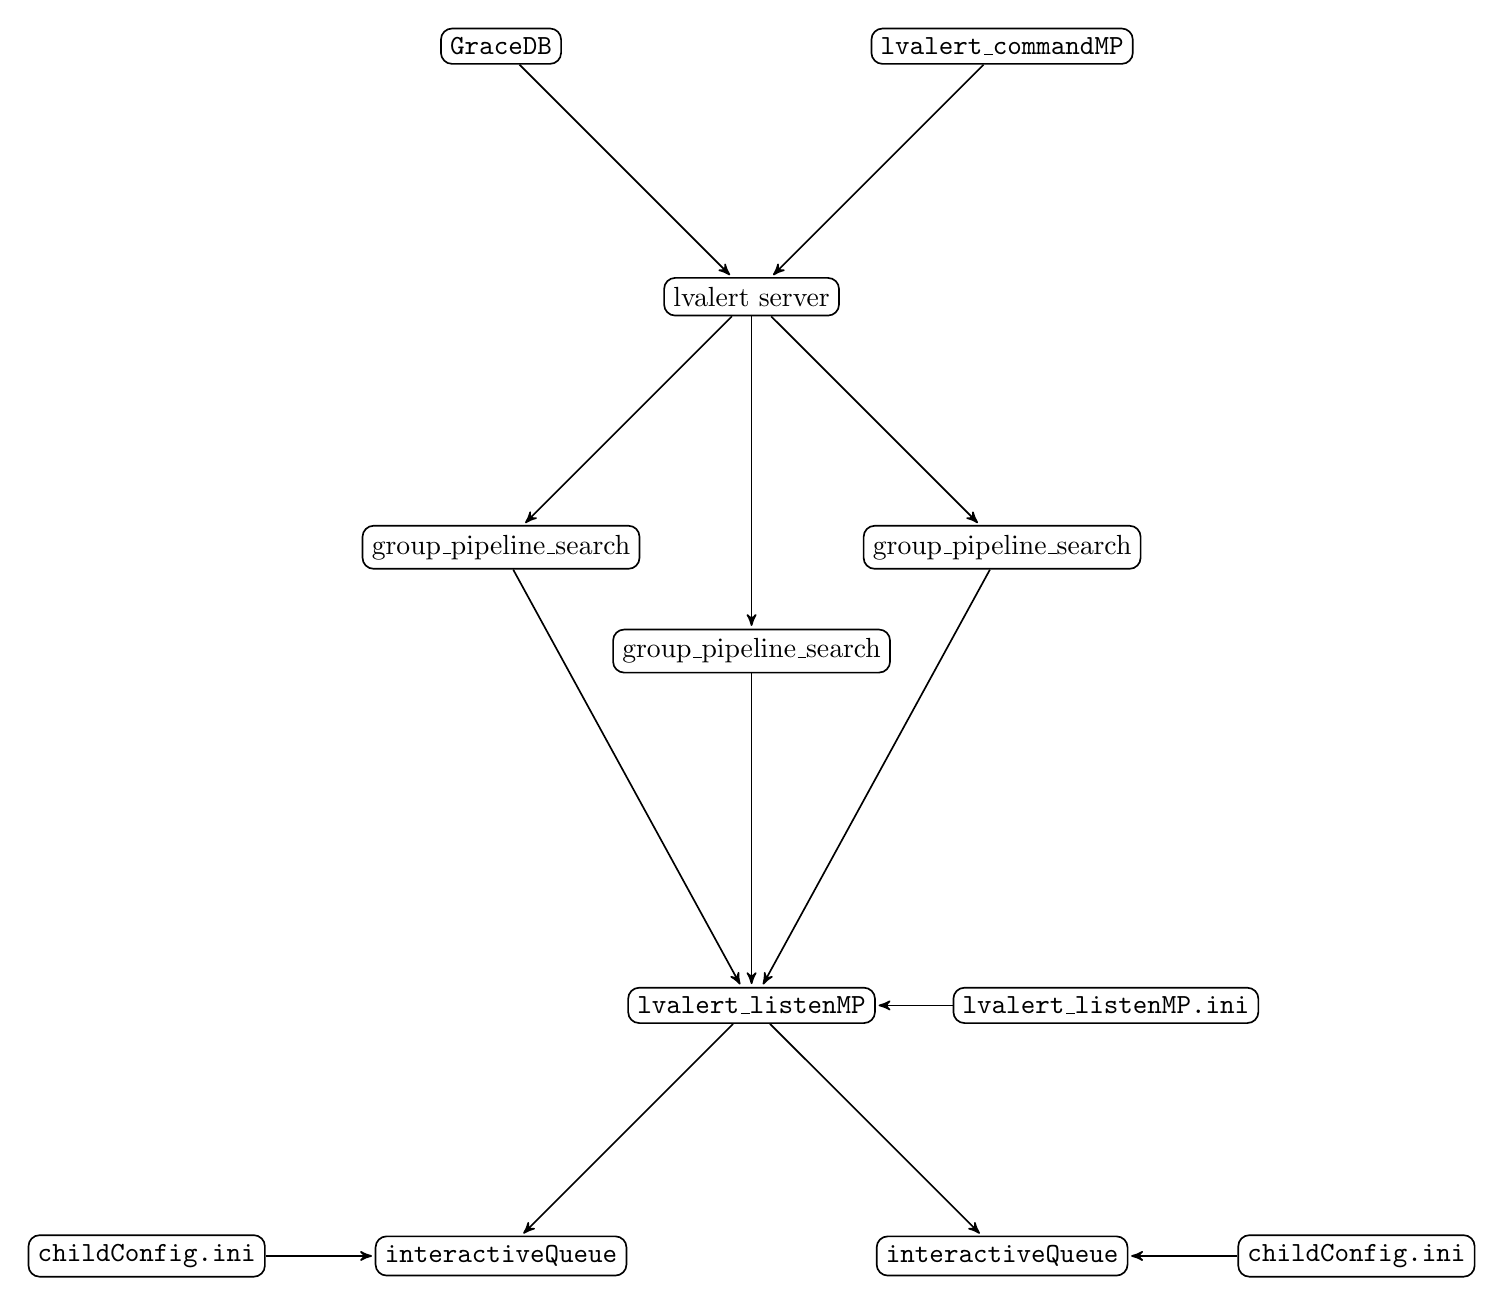
\begin{tikzpicture}[->,>=stealth', shorten >= 1pt, auto, node distance=4.50cm, semithick]
        \tikzset{
           server/.style={
                        rectangle,
                        rounded corners,
                        draw=black,
                        fill=none,
                        text=black
                       },
           lvalertNode/.style={
                        rectangle,
                        rounded corners,
                        draw=black,
                        fill=none,
                        text=black
                       },
           mpPipe/.style={
                        rectangle,
                        rounded corners,
                        draw=black,
                        fill=none,
                        text=black
                       },
           lvalertMP/.style={
                        rectangle,
                        rounded corners,
                        draw=black,
                        fill=none,
                        text=black
                       },
           config/.style={
                        rectangle,
                        rounded corners,
                        draw=black,
                        fill=none,
                        text=black
                       },
           childProc/.style={
                        rectangle,
                        rounded corners,
                        draw=black,
                        fill=none,
                        text=black
                       },
                 };
    %--------------------
        \node[server]      (lvalertServer)                                {lvalert server};

        \node[server]      (GraceDB)       [above left of=lvalertServer]  {\GraceDB};
        \node[lvalertMP]   (lvalertCmd)    [above right of=lvalertServer] {\lvalertCommandMP};

        \node[lvalertNode] (nodeA)         [below left of=lvalertServer]  {group\_pipeline\_search};
        \node[lvalertNode] (nodeB)         [below of=lvalertServer]       {group\_pipeline\_search};
        \node[lvalertNode] (nodeC)         [below right of=lvalertServer] {group\_pipeline\_search};

        \node[lvalertMP]   (lvalertMP)     [below of=nodeB]               {\lvalertListenMP};
        \node[config]      (lvalertConfig) [right of=lvalertMP]           {\lvalertMPini};

        \node[childProc]   (childProc1)    [below left of=lvalertMP]      {\interactiveQueue};
        \node[config]      (childConfig1)  [left of=childProc1]           {\childConfigini};
        \node[childProc]   (childProc2)    [below right of=lvalertMP]     {\interactiveQueue};
        \node[config]      (childConfig2)  [right of=childProc2]          {\childConfigini};
    %--------------------
        \path (GraceDB)       edge (lvalertServer)
              (lvalertCmd)    edge (lvalertServer)

              (lvalertServer) edge (nodeA)
              (lvalertServer) edge (nodeB)
              (lvalertServer) edge (nodeC)

              (nodeA)         edge (lvalertMP)
              (nodeB)         edge (lvalertMP)
              (nodeC)         edge (lvalertMP)

              (lvalertConfig) edge (lvalertMP)

              (lvalertMP)     edge (childProc1)
              (lvalertMP)     edge (childProc2)

              (childConfig1)  edge (childProc1)
              (childConfig2)  edge (childProc2);
    \end{tikzpicture}
    \caption{The flow of \alert messages between processes.}
    \label{fig: alert flow}
\end{figure}

\begin{figure}

\begin{verbatim}
queue = \SortedQueue()
queueByGID = {} <--- explain why we have both queue and queueByGID

while True:
    is there a new alert in the mpPipe?
        parseAlert( queue, queueByGID, alert, timeReceived )

    clean up / manage queue

    if queue[0].has_expired:
        item = queue.pop( 0 )
        item.execute() <--- show how QueueItems are structures and how execute() is delegated to Tasks
        if not item.complete:
            queue.insert( item )

    wait for a small amount of time before checking again
\end{verbatim}

\FIXME{use a flow-chart instead of pseudo-code!}

    \caption{work flow within \interactiveQueue}
    \label{fig: interactiveQueue}
\end{figure}

\begin{figure}

\begin{verbatim}
parseAlert must return an integer representing the change in the number of completed QueueItems in queue.
Otherwise, all bets are off. However, we should show how event_supervisor accomplishes this.
\end{verbatim}

\FIXME{use a flow-chart!}

    \caption{figure showing what happens within \parseAlert as it is written within \eventSupervisor}
    \label{fig: parseAlert}
\end{figure}

%------------------------

\section{suggested extensions}
\label{sec: suggested extensions}

\begin{itemize}
    \item{walk through \eventSupervisor \parseAlert and how it standardizes \_\_init\_\_ API and the relation to sub-modules and config files.}
    \item{walk through how \eventSupervisor extends \Task object to send emails as part of the the execute method, etc}
    \item{walk through the \texttt{bayestar} module within \eventSupervisor to demonstrate class extensions for ``well behaved'' follow-up processes.}
    \item{a suggestion of how \approvalProcessor might accomplish it's goals using the \SortedQueue architecture. Essentially, this becomes a scheduler (like Condor's queue) but with limited scope and functionality}
\end{itemize}

%-------------------------------------------------
\end{document}
%-------------------------------------------------
